\section{Heat Transfer Simulation for Modeling Realistic Winter Sceneries}

While many of the previously presented papers strictly deal with erosion in combination with evaporation and sedimentation alone, the temperature is mostly assumed to be constant. In some simpler cases it is not take into account at all. In paper presented in this chapter, exactly that often "overlooked" topic becomes the primary focus of the calculations.

To allow more complex thermal calculation for simulating a natural environment, one needs to take a lot of different influences and physical processes into account. The existing methods prior to this paper primarily rely on one of those three approaches for calculating winter scenarios for example:
\begin{itemize}
	\item Particle based snow accumulation
	\item Surface displacement methods
	\item Ice growth
\end{itemize}

The name of these methods basically already implies what they fundamentally do:

The particle based accumulation methods evaluate the trajectory of snowflakes (blown by the wind) colliding with the surface \cite{nishita1997modeling}. In an alternative approach the stochastically generated snowflakes are "shot up in the sky" and the calculations are done recursively \cite{fearing2000computer}. Non of these methods are truly physics-based and both of them includes solving Navier-Stokes \cite{feldman2002modeling} or the Bolzmann equations \cite{wang2006real}. The only physics based system mentioned, works on basis of vortex fields and incorporates melting snow, but leaves the weather completely aside.

The surface displacement methods basically only calculate the hight of the accumulated snow falling on a specific spot. This can easily be done by using the depth buffer \cite{ohlsson2004real} or through dissipating calculated ambient occlusion with illumination \cite{foldes2007occlusion}. Another very efficient variant of this approach is done by using hight span maps and heavily relies on a statistical model for snow accumulation derived from observations in nature \cite{haglund2002snow} \cite{festenberg2009geometric}.

Calculating ice growth is not used so widely. Some methods simulate ice crystal formation over objects by using a phase field method \cite{kim2003visual}. Another more sophisticated hybrid-approach combines those phase filed methods with fluid simulation and procedural defused limited aggregation \cite{kim2004hybrid}.

\subsection{The newly proposed approach}
Like many other methods, the approach presented in this paper \cite{benes2001layered} also relies on a voxel grid. Like for so many other authors before mentioned, the challenge is to find the right balance between a high-resolution grid which is able to capture small details, and a large scale grid which requires less memory and computational effort.

Here this problem is handled by evaluating the evolution of temperature of every voxel, taking into account changing weather and environmental conditions (and therefore temperate) over time. After that a heightfield is generated for the surface representation, from the hight of snow stored in the according voxel \cite{benes2001layered}.

\begin{figure}[htb]
	\centering
	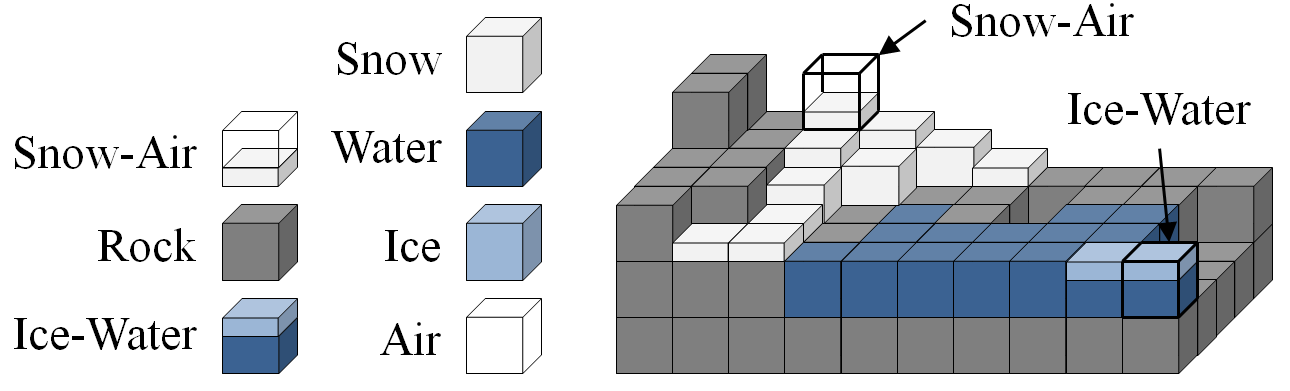
\includegraphics[width=\linewidth]{BF01/84941_1.png}
	\caption{Material types available in this system}
	\label{fig:materialtypes}
\end{figure}

The data structure used for the calculation consists of a grid of voxel, where for each voxel one (or two) materials (see figure \ref{fig:materialtypes}), the temperature and the percentage of solid material are stored along with energy exchange over time. Since some voxel can contain two materials at once (e.g. ice and water or snow and air), these voxel need to be evaluated more carefully. Phase transitions are more likely to occur in those "mixed" voxel than in any other one.

\subsection{The calculation process}
In the calculation technique itself its rather complicated and it will only by presented as an overview here (see figure \ref{fig:calcpipeline}). Due to it's highly physically-based background the results are very accurate, but not meant to be used for real-time calculations.

The necessary calculations for this approach is performed in four different steps:
\begin{enumerate}
	\item Compute environment parameters
	\item Simulate snowfall and accumulation
	\item Compute thermal (and energy) transfer between voxel
	\item Computer phase-change for affected voxel
\end{enumerate}

\begin{figure}[htb]
	\centering
	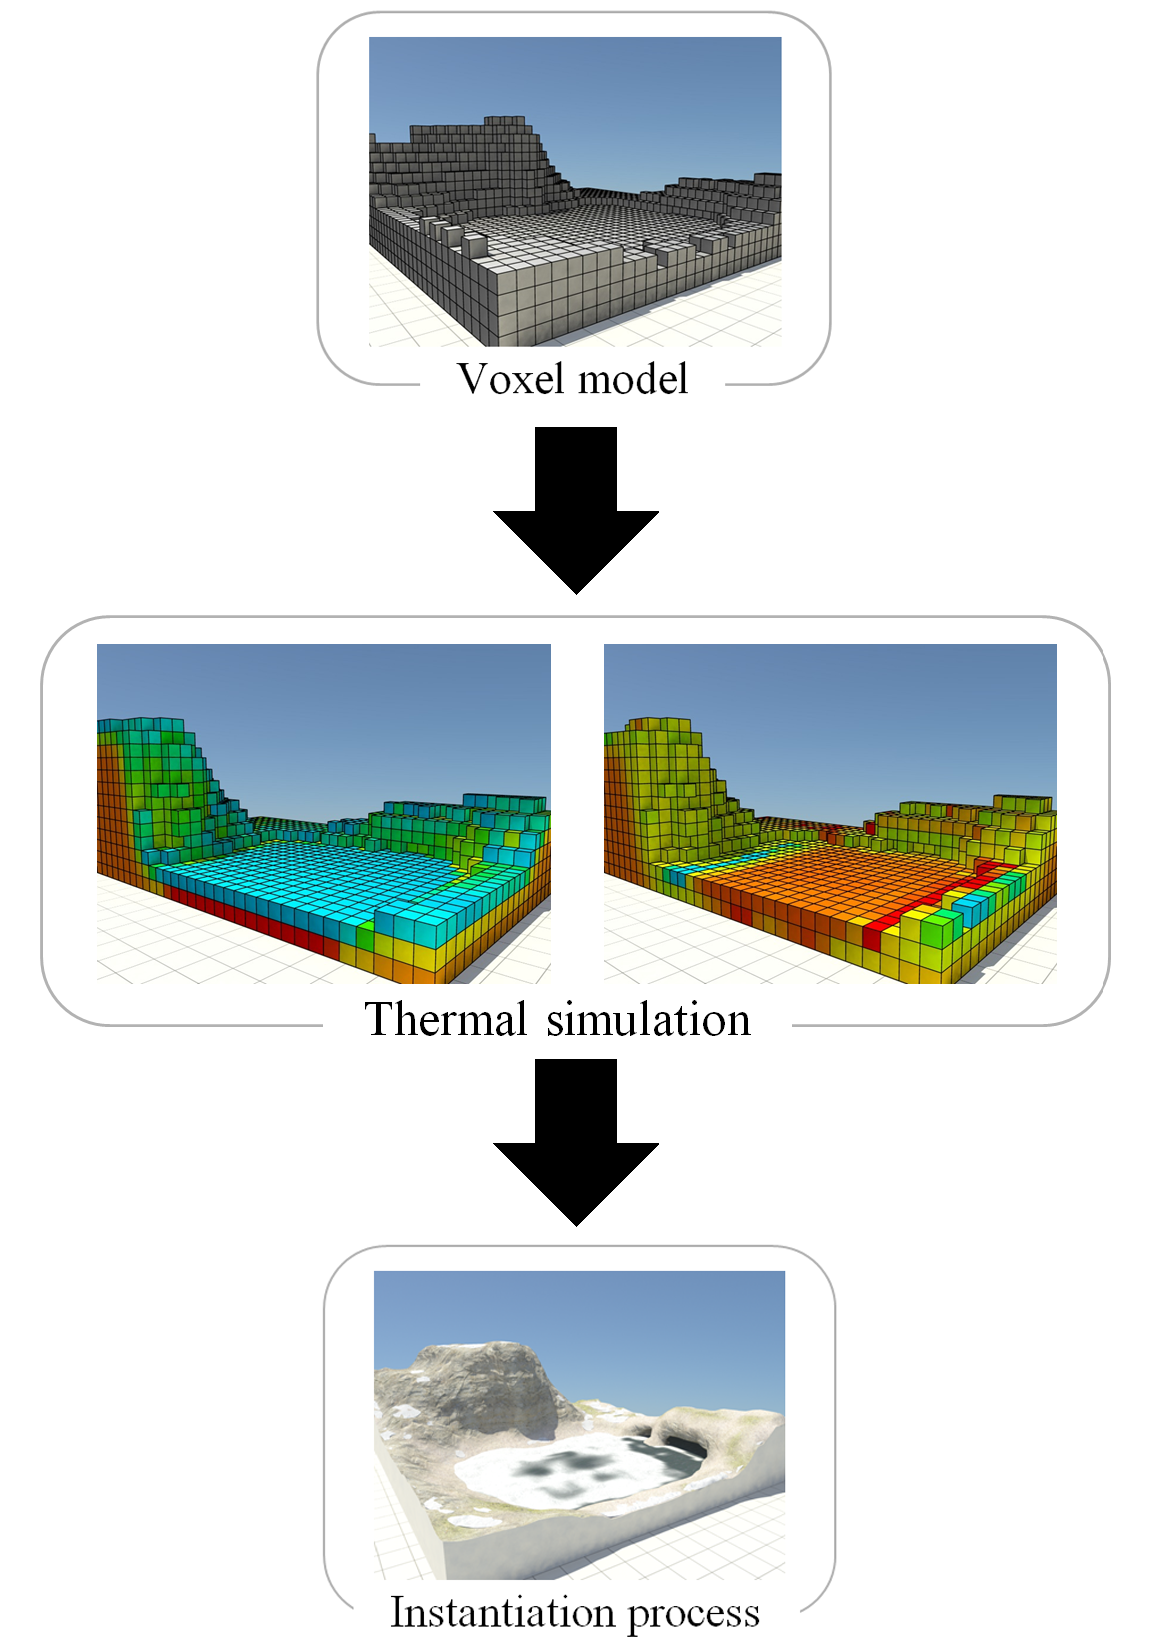
\includegraphics[width=\linewidth]{BF01/sem_heat2_merged.png}
	\caption{The calculation pipeline}
	\label{fig:calcpipeline}
\end{figure}

These five materials are key to all calculations performed here: Rock, Ice, Water, Snow, Air. Every material has it's own constraints and attributes. Some of this attributes are mass density, specific heat capacity, thermal conductivity, emissivity, melting temperature, etc.

In addition to the materials itself, there are a number of global factors and attributes needed for the calculation, which are defined in the environmental model. This model defines the development and change of weather over time. Weather itself is defined as air temperature, dev point, the amount of snowfall, the cloud cover as well as information about day- and night-cycles.

\begin{figure}[htb]
	\centering
	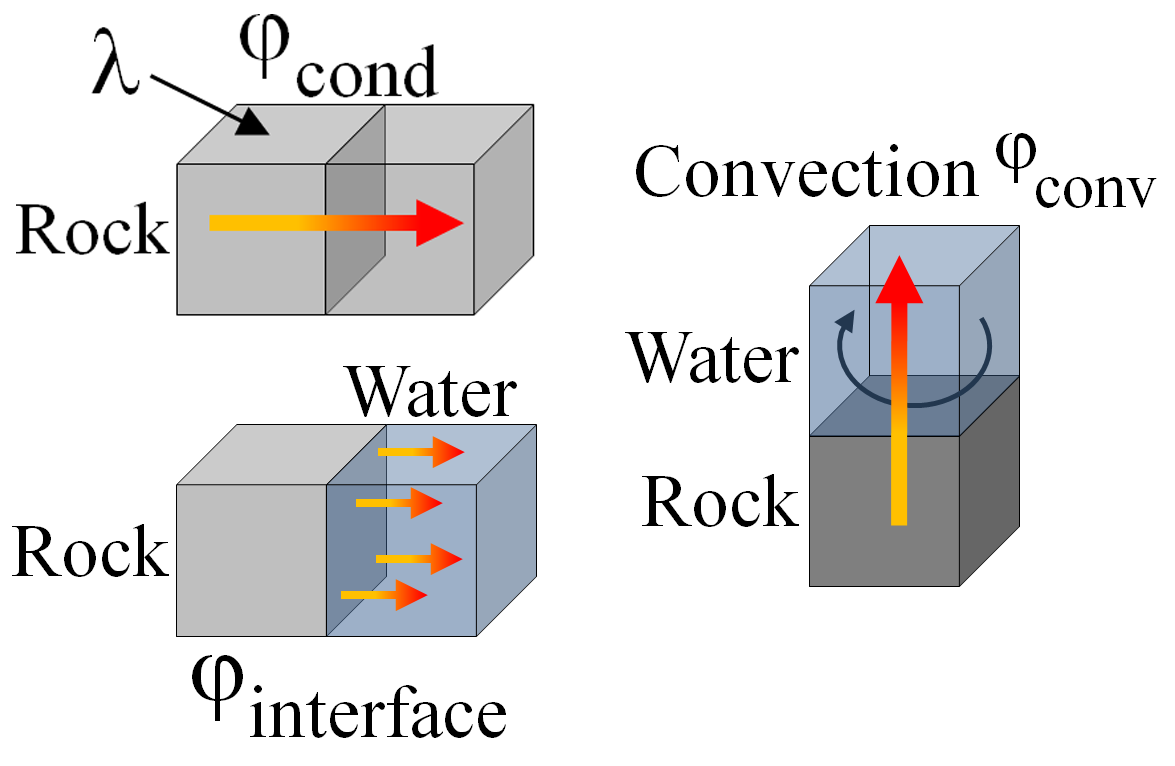
\includegraphics[width=\linewidth]{BF01/sem_heat_merged1.png}
	\caption{Calculations to be done inner- and cross-material heat transport}
	\label{fig:calcheattransport}
\end{figure}

All thermal transfers happening in the simulation can be categorized as one of the following types (for exaples see figure \ref{fig:calcheattransport} and figure \ref{fig:calcradiation}):
\begin{itemize}
	\item Conduction is the heat-transfer between to media in contact
	\item Convection takes place within fluid materials and on the boundaries to solid material
	\item Radiation is defined as energy emitted as (electro-magnetic) waves from a surface
\end{itemize}

Without going too much into detail here it can again be stated that these calculations are based on several physics-equations and take a lot of detailed factors and influences as well as properties into account (see figure \ref{fig:calcsystem}). For example can the warming up of a surface from the energy (heat) impact through sun-rays not only be assumed to be constant. In this computational model the temperature of the sky itself is needed to get an result. This temperature does depend on the temperature of the air at this time, and the dew point temperature. In addition to that the degree of the sundays hitting the surface is evaluated. If the sky is not assumed to be cloudless, the amount of vapor in the air (which is decreasing with the dew point temperature) has also to be taken into account. After that, the actual filtering of the sun-rays through one or more clouds can be applied. Another good example is the calculation of indirect heat, which is reflected from nearby surfaces and can effect snow-melding in the mountains in nature for example.

\begin{figure}[htb]
	\centering
	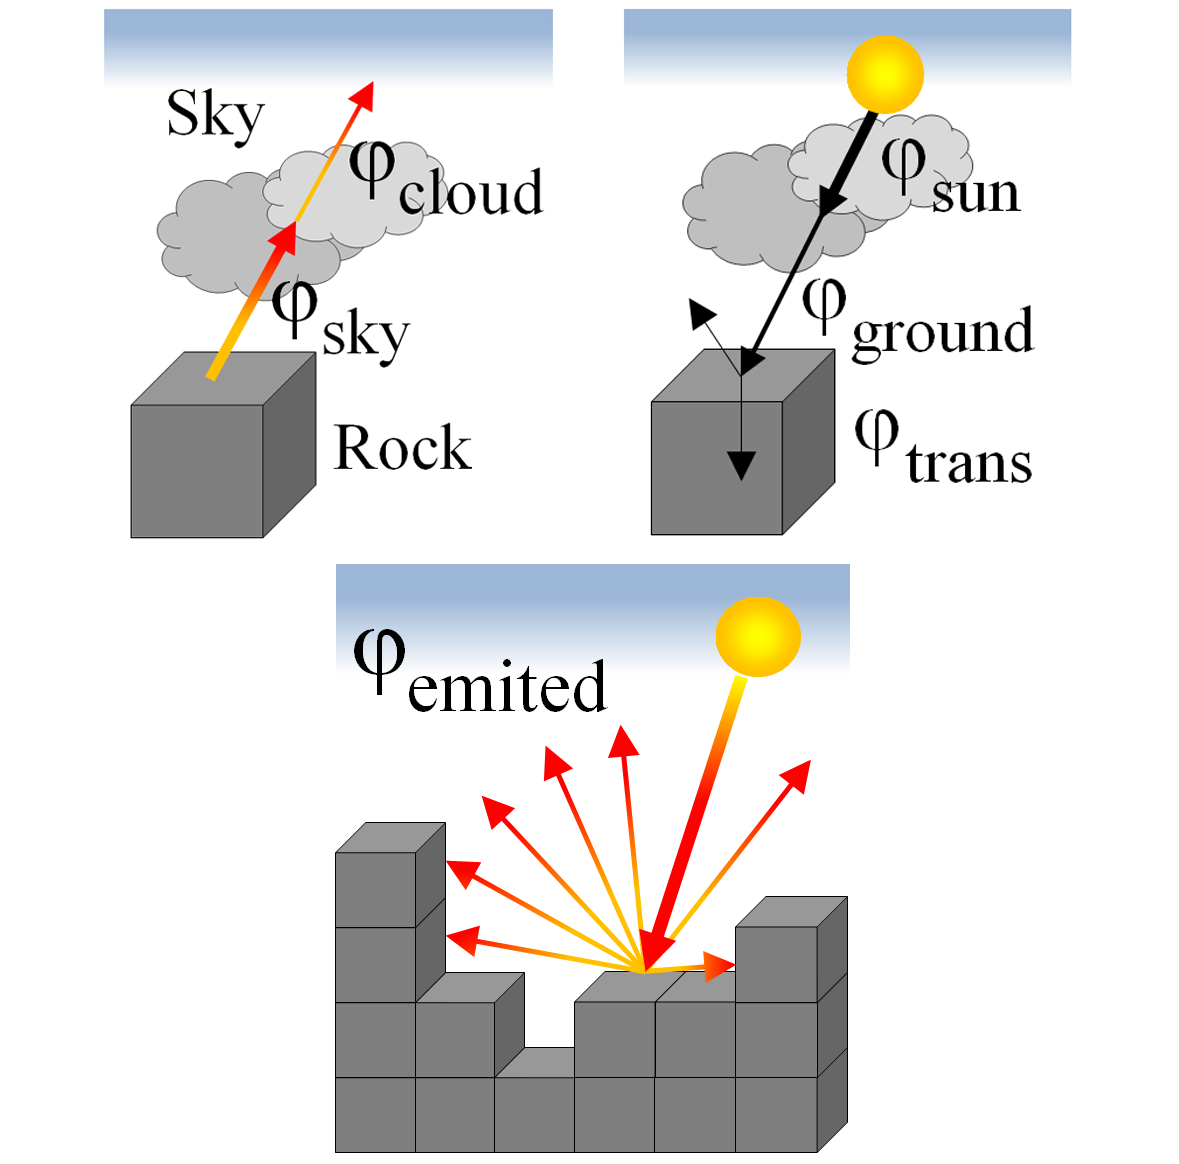
\includegraphics[width=\linewidth]{BF01/sem_heat_merged2.png}
	\caption{Calculations to be done for light and radiation}
	\label{fig:calcradiation}
\end{figure}

\begin{figure}[htb]
	\centering
	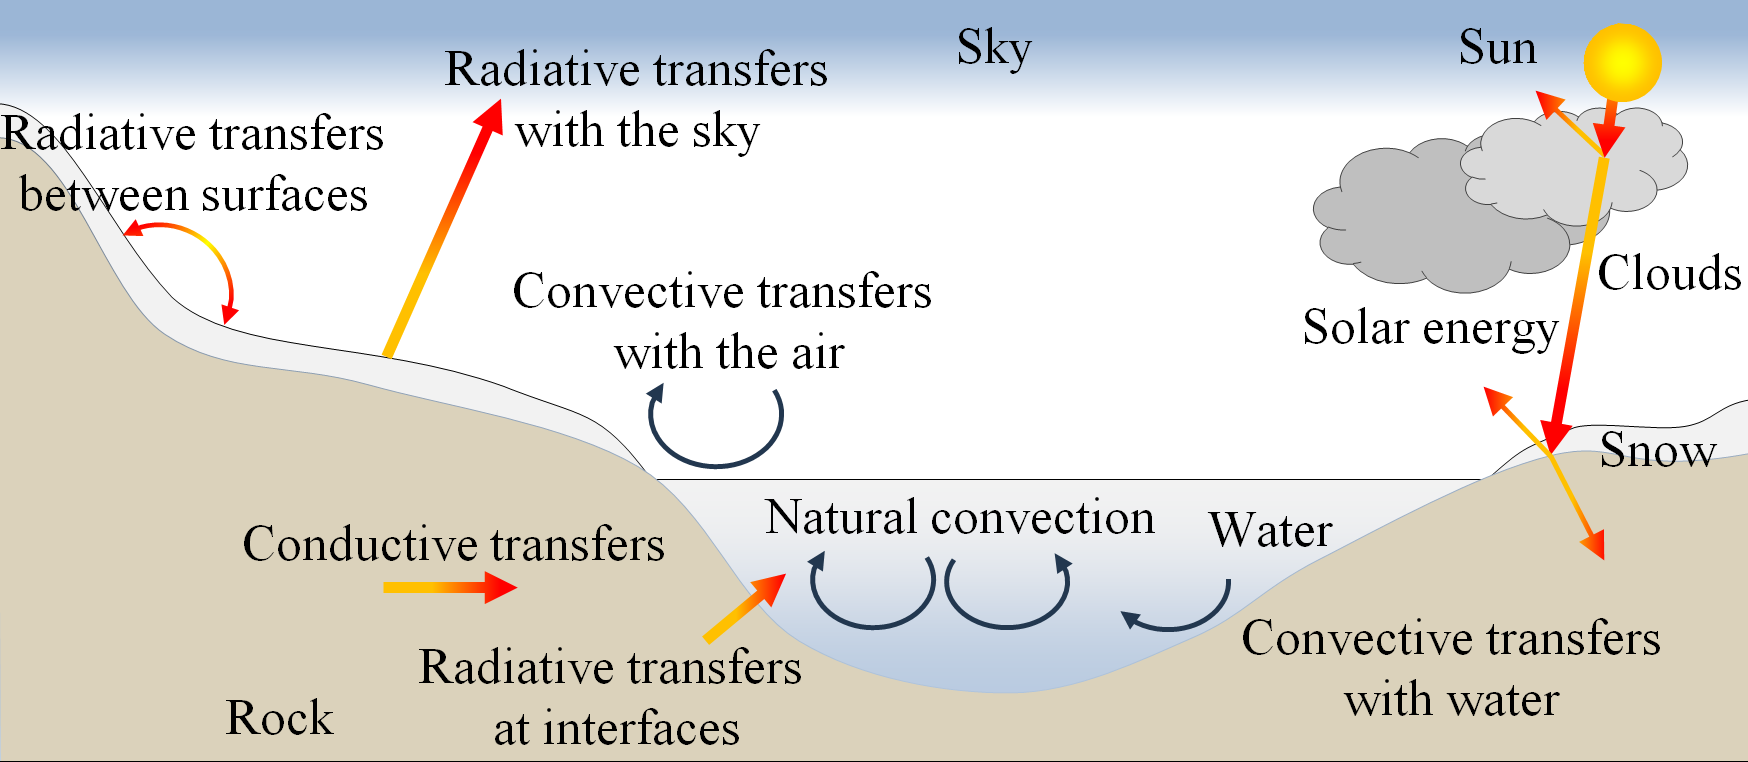
\includegraphics[width=\linewidth]{BF01/8904_1.png}
	\caption{Illustration of the quite complex calculation system}
	\label{fig:calcsystem}
\end{figure}

For the phase changes from one material to another, a fusion temperature is defined. If this temperature is reached, the (partial of complete) transition of this voxel is performed. Since some aspects go ever further into detail than this paper already does, things like the dynamics of flowing water is approximated in the calculations. This would have to be done in addition to computing the absorption and evaporation of water through solid ground (rock) and therefor distinguishing between dry and wet rocks. Also the possibility of flowing water freezing during movement due to slow flowing speeds and low temperatures of the ground, is not take into account here. Another interesting physical phenomenon included in this model's calculations are different temperatures within a lake or even a puddle of water. Since the weight of water changes a little with its temperature, and the sun generally warms the upper layer of a lake more than the lower parts of it, a lake or pond can come times be decided into more than one different temperature zones (see figure \ref{fig:waterconvection}).

\begin{figure}[htb]
	\centering
	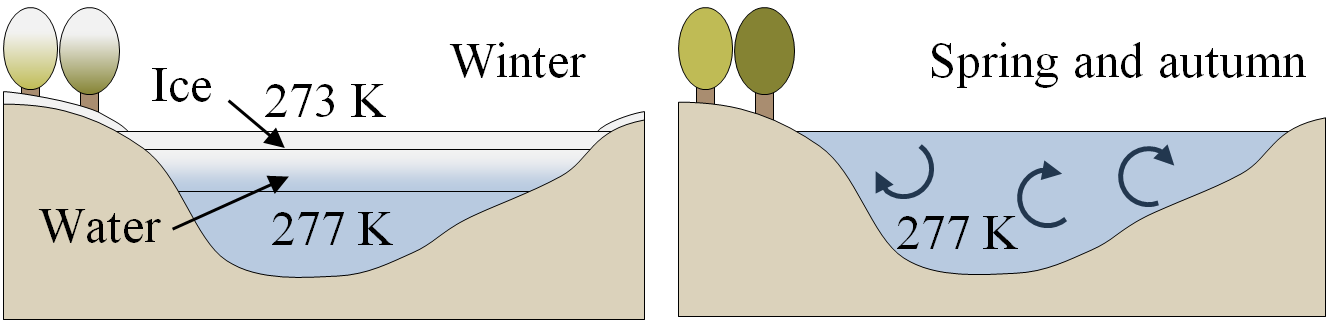
\includegraphics[width=\linewidth]{BF01/h_1.png}
	\caption{Different water temperatures and convection}
	\label{fig:waterconvection}
\end{figure}

For generating Snow on a surface-level or freezing water resulting in ice, a more approximated technique is used. Snow on the surface is simple represented by a textured hight field, which is obtained by the elevation of the vertex grid at that point. For freezing water inside a like as it can be seen in figure \ref{fig:iceinwater}, two hight fields are generated: one for the upper and one for the lower surface of the developing ice. The the separation of those, the thickness of the ice-layer can be controlled.

\begin{figure}[htb]
	\centering
	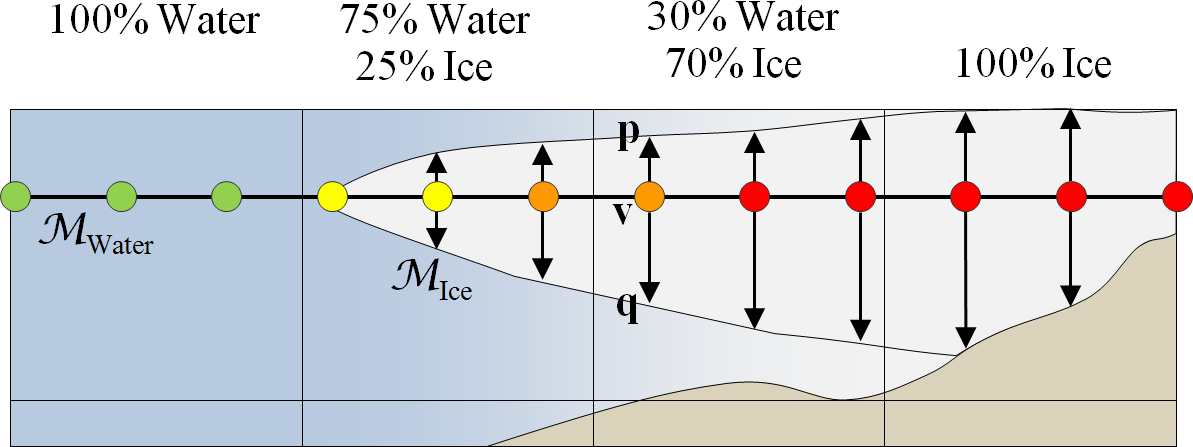
\includegraphics[width=\linewidth]{BF01/i_1.png}
	\caption{Calculation of ice forming in water}
	\label{fig:iceinwater}
\end{figure}

\subsection{Performance}
As is can easily be derived from the complexity of the calculations done in this approach, this technique was never meant to be performed in real-time. Although the time step can be set relatively large, since thermal effects occur much slower than many other natural phenomena, the time needed for the calculations is still quite high.

Nevertheless the paper include one relatively simple example of a landscape simulation, along with the time it took to compute. The implementation used was written in C++ and run on an Intel Dual-Core processor with 3GHz and 3GB RAM. On this hardware the calculation for a nine day weather model on a grid of 3.2 million voxel tool about 5 hours \cite{benes2001layered}.